PX4 provides a default \acs{uav}, the iris. 
The iris is a quadcopter that has multiple control options, providing redundancy and flexibility. 
It has a built-in radio for real-time mission monitoring, data logging and control. 
For controlling the \acs{uav} it has powerful cross-platform ground station/mission planning and 
analysis software that runs on Windows, \acp{os} X and Linux, providing simple point-and-click programming 
and configuration. And finally Maybe the most important feature for a developer: failsafe programming 
options in the event of lost control signal, \acp{gps}, or low battery conditions \cite{arducopter:iris}.

\begin{figure}[ht]
    \centering
    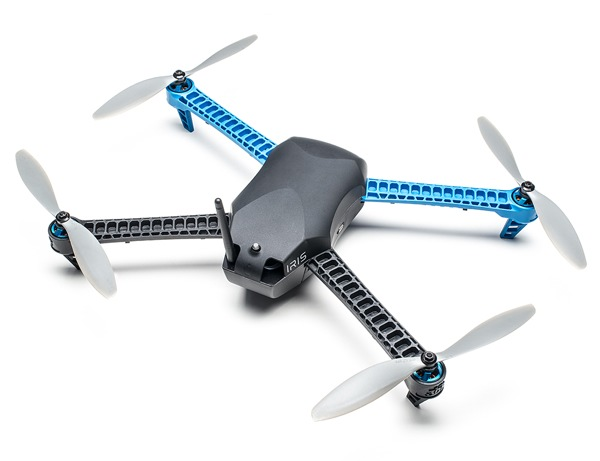
\includegraphics[scale=0.4]{iris.jpg}
    \caption[Iris drone]{Iris drone}
\end{figure}

Using xarco files a developer is able to add components to this \acs{uav}. 
In this project it is able to spawn up to 10 \acp{uav}. This limitation does not come from the xarco files
but from this project which will be later clarified
As a generic solution the project contains a generate\_launch script 
that can accept a parameter for n amount of \acp{uav}. 
This script is written in bash so the argument can be passed in the command line. 
It generates a launch file as a string, and then writes this launch string to a file named 
“smartuavs.launch” inside the launch folder. This will later be further detailed in the simulation container.

In the project a \acs{3d}-camera is added using a components snippets from the PX4 github repository. The \acs{3d} camera has 
multiple topics where it publishes to where it publishes data.
